\newpage

\chapter{関連技術}
本章ではプロシージャルモデリングおよび遺伝的アルゴリズムについての詳細および関連研究について紹介する.

\section{プロシージャルモデリング}
\subsection{概要}
\ プロシージャルモデリングとは,研究背景にも簡単に記載した通り,数式などの計算処理を組み合わせてモデリングを行う手法である. CG 分野で非常に幅広く活躍している技術であり,単なるオブジェクトだけでなく,計算機の能力にもよるがエフェクトや物理演算といったリアルタイムでの変化が必要なものに対しても用いられている.近年ゲーム業界では,オープンワールドのような広大なマップを作成するのにあたり,特に注目を集めている.

\subsection{関連研究}\label{label:relatedResearch}
プロシージャルモデリングについての研究として,大きく3つに分かれている.


一つ目は,植物\cite{lintermann1999interactive}や地形\cite{smelik2011declarative}といった自然物から城\cite{三浦嘉大2020地理的要素とユーザー自由度を考慮した日本城郭都市のプロシージャルモデリング}やビル\cite{muller2006procedural}などの人工物,煙\cite{xie2022dualsmoke}や火などの一つの状態を持たないパーティクルなど物体表現に焦点を当てた研究である.特に近年物体表現に焦点をあてたものに関して Sketch-base による形状指定することでの生成研究は多い反面,パラメータを手作業で調整するものの研究は数が少ない.その理由としては,研究背景の説明にもある通り,表現をより良くすることによるパラメータ数増大が原因であると考えられる.


次は機械学習と組み合せた研究\cite{DBLP:journals/corr/abs-2010-04548}である.特にこの研究は近年非常に目覚ましい成果を挙げており,その中でも特に顕著なものはゲームにおけるレベルデザインに関する研究である.理由として,モデリングに関する評価を自動テストによってどの程度の難易度であるかを評価できる点にある.


そして最後に紹介するのが,プロシージャルモデリング時の効率的な作成システムに着目した研究である.


koyama らはベイズ最適化を用いた手法である BO as Assistant \cite{koyama2022bo}を提案している.図\ref{fig:boAssistant1}にシステムの実装画面を示す.
この研究では,プロシージャルモデリングにおけるパラメータ操作以外に,3つの提案モデルがベイズ最適化によって生成され,従来のパラメータ操作に加え,そのモデルに対する補間操作を行う事が出来るスライダーが追加されている.
また生成状況に合わせて再提案のボタンを押す事で別のモデルが提案されていき,プロシージャルモデリングのパラメータ操作を複数同時に行えるため,その分効率的なモデリングが出来たとされている.一方で,ベイズ最適化のモデリングにおけるパラメータ数に制限があるとされている.

図について
, Design preview は操作が行われるモデルであり,各パラメータのスライダーと Blending slider を動かすことで変化する. Blending slider は各 Suggestion モデルとの補間を行う事が出来,一番右端にスライダーを移動させることで, Design preview が対応する Suggestion モデルと一致する. Regenerating button を押すことで,現在の Design preview が獲得関数が最大になる直近のデータとしてベイズ最適化に適用され, 
再計算された獲得関数にサンプリングし Design preview を除いた上位3つが Suggestions として更新される.
本研究ではこの手法との対照実験を行う.

\begin{figure}[h]
	\begin{center}
		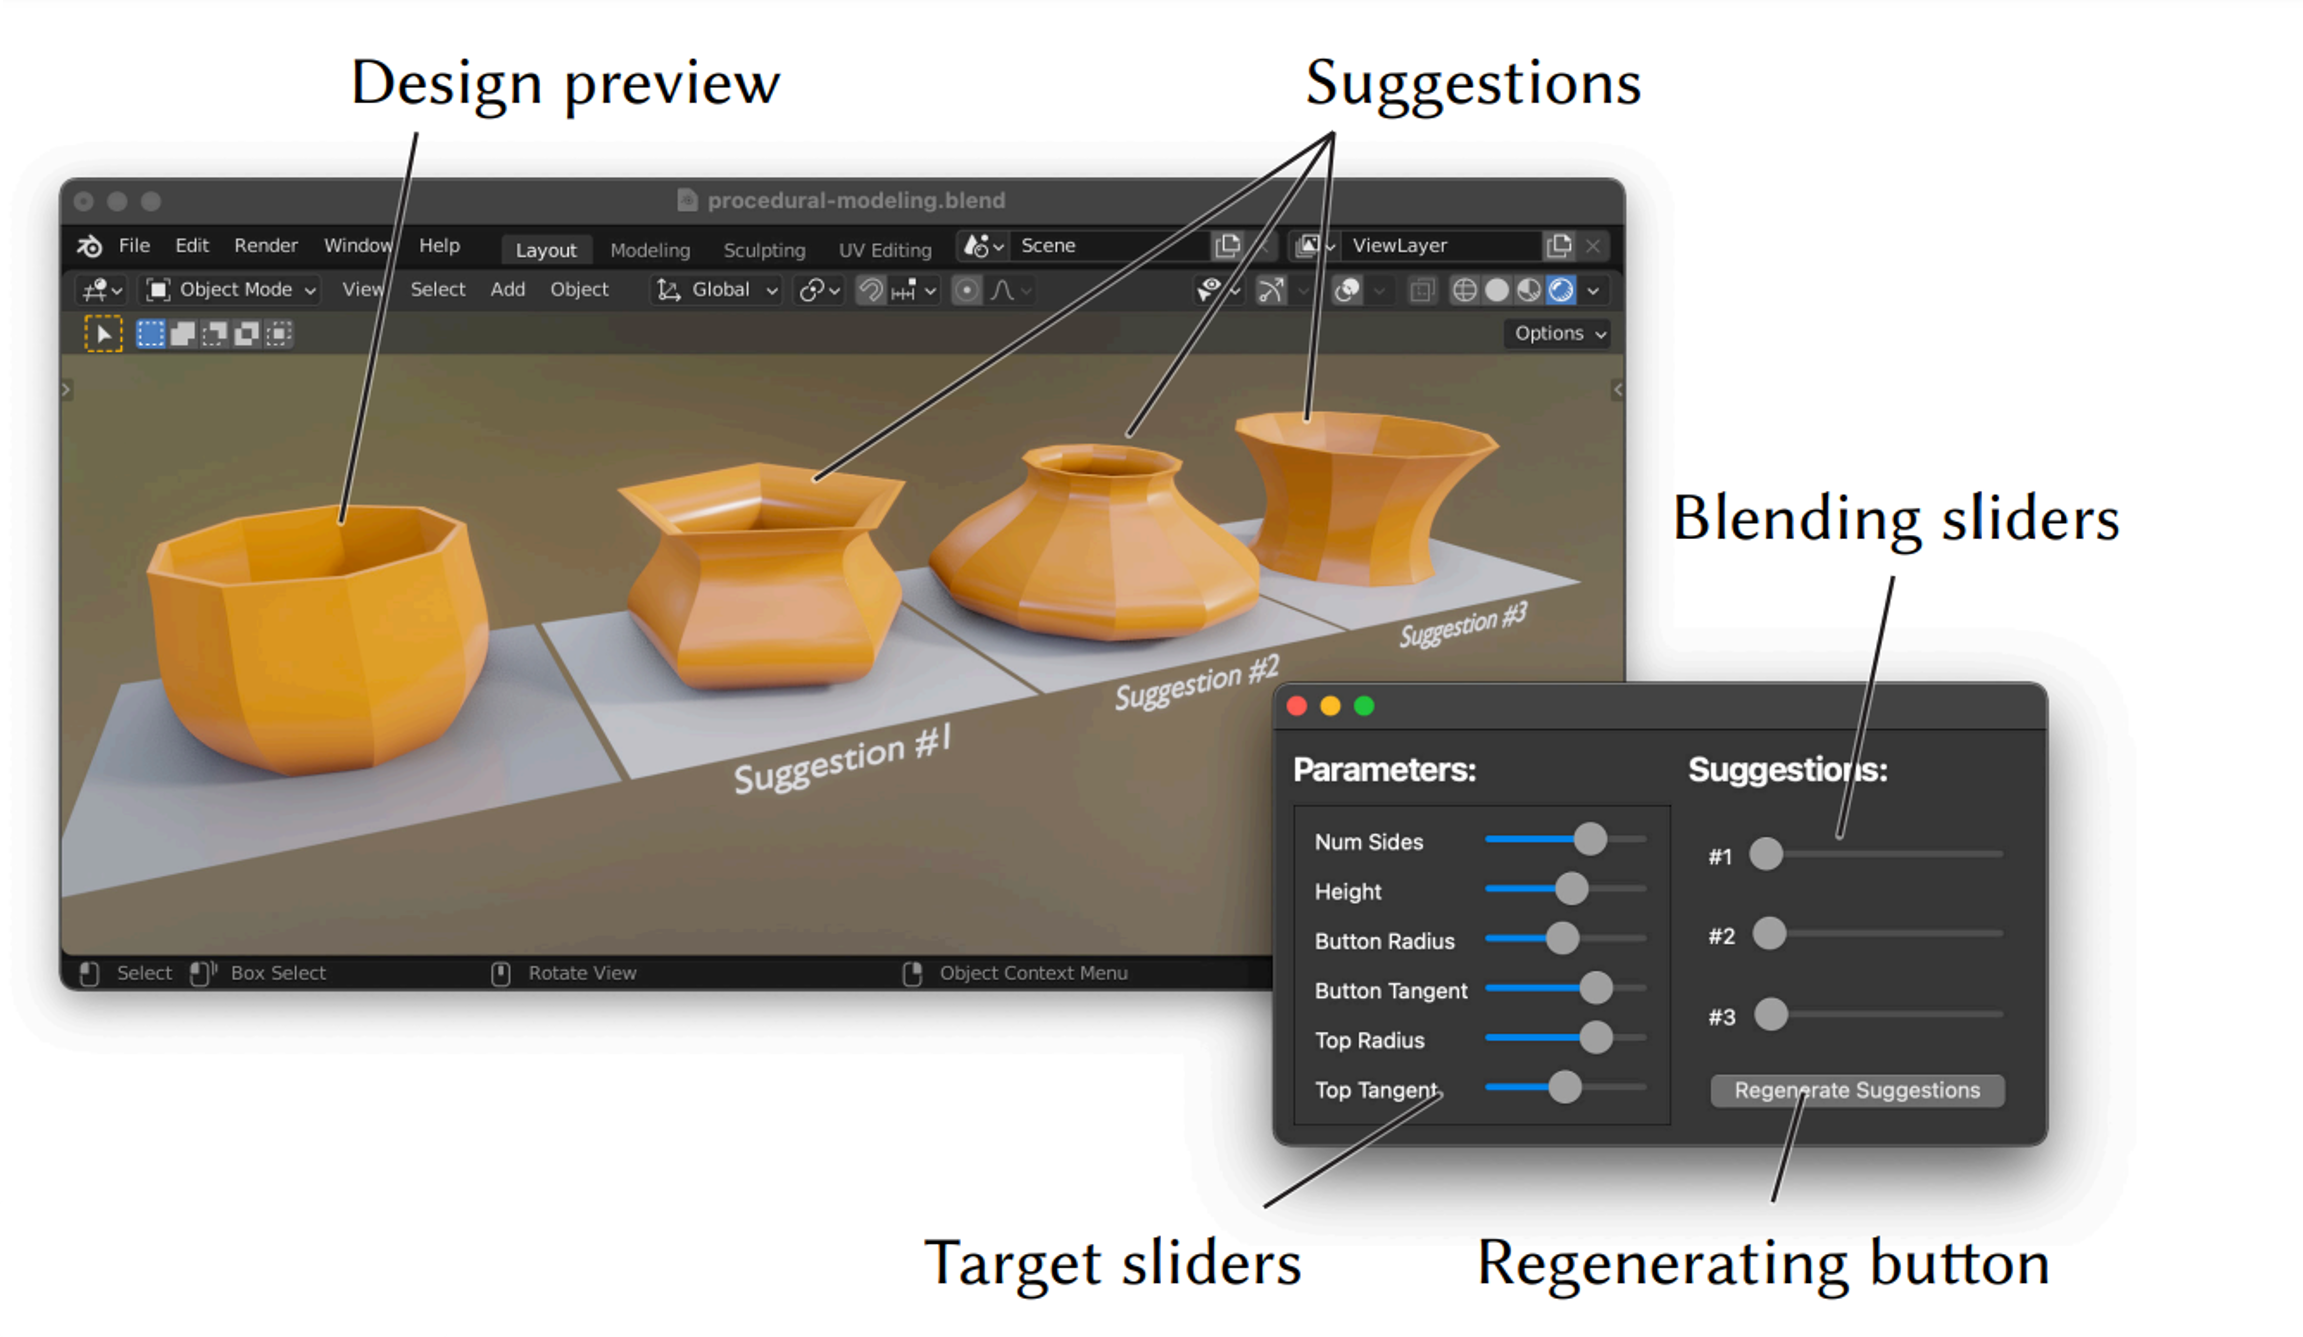
\includegraphics[scale=0.7]{./imgs/boAssistant1.png}
		\caption[BO as Assistant]{BO as Assistant (: 先行研究\cite{koyama2022bo}の Preview Video より引用\label{fig:boAssistant1})}
	\end{center}
\end{figure}


\newpage

\section{インタラクティブ遺伝的アルゴリズム}
  インタラクティブ遺伝的アルゴリズム(Interactive Genetic Algorithm : IGA)とは,ユーザとの対話を用いた遺伝的アルゴリズムである.まず遺伝的アルゴリズムの概要について説明の後,インタラクティブ遺伝的アルゴリズムについての詳しい説明を行う.

\subsection{遺伝的アルゴリズム}
  遺伝的アルゴリズム (Genetic Algorithm : GA)\cite{whitley1994genetic} とは,生物の進化を模倣した組合せ最適化問題のアルゴリズムであり,メタヒューリスティクスとしてよく利用される. 
  
  解の要素の最小単位を遺伝子,遺伝子の集まりである解を個体として表現する.また個体の集合を世代とし,各個体の計算された適応度をもとに選択,交叉,突然変異の3つの操作によって新たな個体群を生成し,次世代の個体集合とする.個体の適応度評価と前述の3操作によって,1世代において適応度の高い遺伝特性を持つ個体が増加する.それによって最適解に近づいてく.
  
  個体の基本的なエンコーディング方法として,バイナリ型,順列型,実数型,整数型がある.本研究では特に実数型について取扱うため,以降実数型を前提とした説明を行う.

\subsubsection{選択}
  選択\cite{blickle1996comparison}は自然淘汰をもとにした操作であり,個体の適応度にもとづき次世代に残される個体を選ぶものである.以下のものがあげられる.

\begin{itemize}
	\setlength{\leftskip}{25mm}
	\item[エリート選択\cite{murata1996multi} : ]世代における適応度の最も高い個体を他の操作を行わず次世代に残す手法である.

	\item[トーナメント選択 : ]個体群からランダムに決められた数(: トーナメントサイズ)取り出し,
	その中で適応度の最も高い個体を選択する手法である.
\end{itemize}


\ これら選択操作によって,適応度の高い個体,つまり世代の中で評価の高い個体の遺伝子が次に引き継がれることによって,前世代において評価の高い遺伝子特性の一部が次世代に引き継がれる.


\subsubsection{交叉}
交叉は生物の交配をもとにした操作であり,2つの個体から新たな2つの個体を生成するものである.遺伝子の種類が有限集合であるバイナリ型や一部の整数型は,生物の遺伝子を模倣した交叉である二個体における遺伝子の交換操作によってなされる交叉が利用できるのに対して,無限集合である実数型は利用できない.遺伝子の交換による交叉だけでは,二つの遺伝子の間に最適となる遺伝子があったとしても探索出来ないので,有限集合における交叉方法では探索が不十分である.そこで,以下のものが挙げられる.
\begin{itemize}
	\setlength{\leftskip}{0mm}
	\item Blend Clossover alpha (BLX-$\alpha$) : 
        \begin{enumerate}\setlength{\leftskip}{5mm}
            \item[] 2つの親個体からなる区間の両端$\alpha$倍した領域においてランダムな子個体を生成する.
        \end{enumerate}
        
	\item Unimodel Normal Distribution Crossover (UNDX)\cite{ono1999robust} : 
        \begin{enumerate}\setlength{\leftskip}{5mm}
            \item[] 3つの個体を用いた交叉であり,そのうち二つを直線で結び,残りの個体と直線との距離を広がりに持つような多次元正規分布によって子個体を生成する.
        \end{enumerate}
 
        \item 多親交叉 Real-coded Ensemble Crossover (REX)\cite{小林重信2009実数値} : 
         \begin{enumerate}\setlength{\leftskip}{5mm}
            \item[] 複数の親個体を用いた交叉であり,その親の重心を取ったのち,全ての親に対し任意の確率分布に従う確率変数を重みとして移動させたものを新たな子個体として生成する.UNDXを多親個体として一般化したものに相当する.
        \end{enumerate}
\end{itemize}

\subsubsection{突然変異}
個体の遺伝子を変化させる操作で,局所探索になることを防ぐ.
乱数によって他の取りうる値に変化させる.また,突然変異率を上げすぎるとランダム探索となり,
収束しなくなるため,高くても数\%に設定されることが多い.

\subsection{IGA と GA の違い}
図\ref{fig:iGAOverView}にインタラクティブ遺伝的アルゴリズムの概略図を示す.
インタラクティブ遺伝的アルゴリズムが通常の遺伝的アルゴリズムと違う点は,適応度計算が計算機によって自動で行われるか,ユーザが行うかの違いである.
\begin{figure}[h]
	\begin{center}
		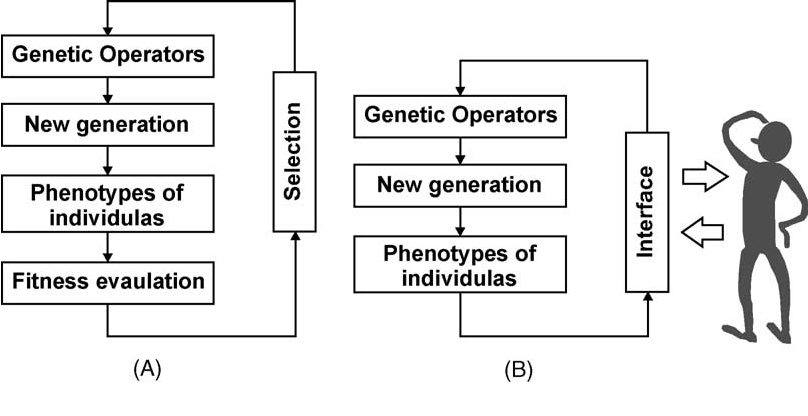
\includegraphics[scale=0.5]{./imgs/iGA_overview2.png}
		\caption[IGA の概略図]{(A) GA の概略図,(B) IGA の概略図 (: 文献\cite{MADAR20051591}の Figure 1より引用\label{fig:iGAOverView})}
	\end{center}
\end{figure}

遺伝的アルゴリズム自体がメタヒューリスティクスであるため,
人間の認識といった計算機では測れないブラックボックスな問題にも適応する事が出来る.しかし問題点として,計算機ほど素早く適応度の計算を行う事が出来ない.適応度計算は基本的に,複数の選択肢を提示しそれに点数をつけたり,あるいはより単純に良いか悪いかを選択するといった方法で行われる.そのため,遺伝的アルゴリズムがより良い近似解を出すのに必要な個体数や世代数が稼ぐ事が出来ないという点も問題となる.


\subsection{関連研究}
インタラクティブ遺伝的アルゴリズムの研究については人間の負担をどのように減らすかが特に重要視されており,近年では機械学習と組み合わせた研究\cite{gypa2023propeller, li2023quantification}も盛んである.


機械学習を用いない研究としては, wang らの研究\cite{wang2020method}では,KJ 法を用いることであらかじめ探索範囲を絞ることで実現している.また,mikiらの研究\cite{miki2006global}では,複数人で分散的に探索を行うことで一人の負担を減らしつつも,個人個人の意見を考慮しつつの探索を可能にしている.また,その他にも様々な製品\cite{dong2008tile, 竹之内宏2022対話型人工蜂コロニーアルゴリズムを用いたランニングシューズデザインシステム}への活用研究もなされている.しかしそれらの研究について,制限としてインタラクティブ遺伝的アルゴリズムに用いられる遺伝子数,つまりパラメータの数は10個前後であることが多い.

\section{本研究の位置づけ}
本研究ではプロシージャルモデリングにおける操作負担を減らすことが目的となる.そのためにいくつかのモデルを提案することで,より効率的なモデリングの手助けをさせる.そのうえで,既存の最適化手法ではパラメータ数に制限がかかる問題があるが,それをインタラクティブ遺伝的アルゴリズムを用いて解決できないかと考えた.そして,パラメータ数の多い場合ではその分探索範囲を広げるために,従来のような複数の選択肢から選ぶ方法だけではなく,複数の選択肢を補間されたものを選択するシステムの手法を考案した.インタラクティブ遺伝的アルゴリズムと補間操作を組み合わせたシステムによってモデルの提案を行うことに新規性を有しており,より多くのパラメータを持つプロシージャルモデリングに対して時間短縮を行えることを期待する.